\section{Power Node}
\subsection{Introduction}
My goal was to design an MTD device that could be powered by a larger capacity Lithium-Polymer battery cell and integrate on one circuit five different target devices, which could be
\begin{itemize}
    \item PIR (Pyroelectric Infrared Sensor) node, i.e. a motion detection node,
    \item a motor driver with a higher power output 5\,\si{\volt} (e.g. a low power irrigation pump),
    \item an environmental monitoring node (temperature, humidity, air pressure and brightness),
    \item node for connecting higher power devices with external power requirements,
    \item motion sensor, door opening sensor node. 
\end{itemize}
All of these are available on a PCB and depending on the end use, one or more functions are available depending on the soldering of the different parts.


\subsection{Power Node schematic}
\begin{figure}[!htb]
    \centering
    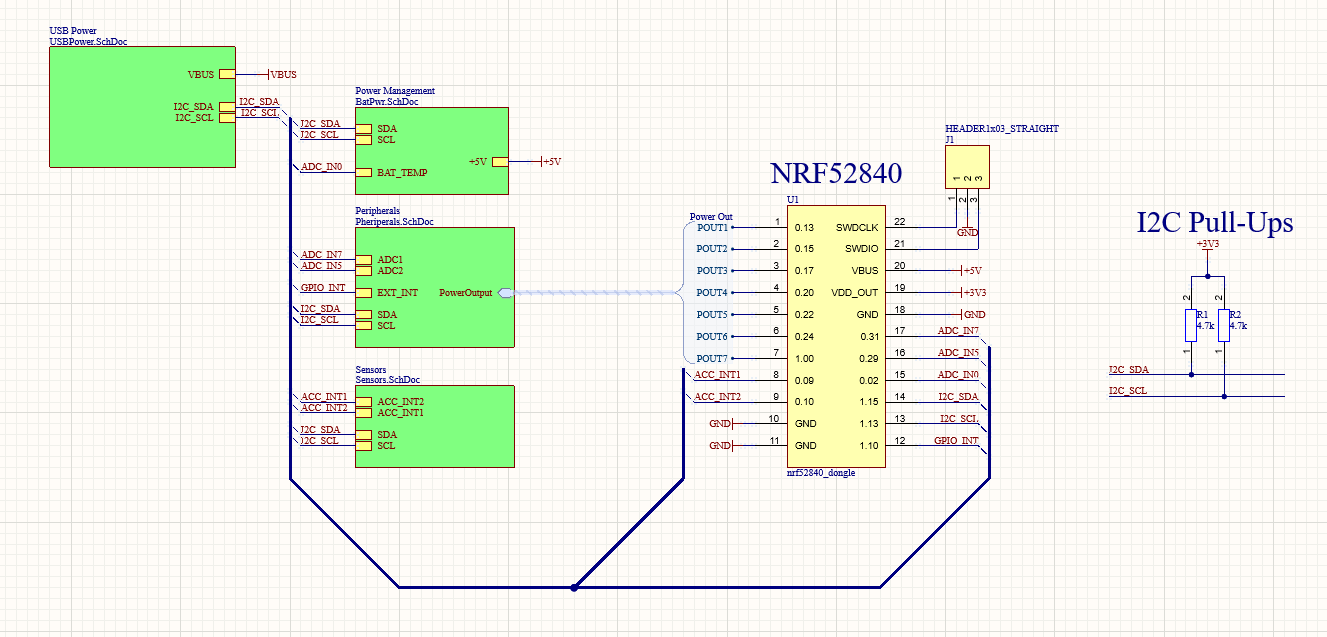
\includegraphics[width=\textwidth]{img/powernode.png}
    \caption{Power Node schematic}
    \label{fig:powernodeschematics}
\end{figure}
\noindent
Figure \ref{fig:powernodeschematics} shows the schematic of this device. From top left down, the first box indicates the USB Type-C charging connector, which allows the device to be operated from an external 5\,\si{\volt} power supply. The I2C bus is used to read the power meter IC. To the right of this block is the charger and the \textit{Battery Protection} (short \textbf{BPS}) circuit to protect the Li-Po battery. The I2C bus is used to access the measured data of another power meter IC, as this is used to provide the microcontroller with information about the status of the voltage source, which can later be used to signal the user when the device needs charging. On the other hand, it is a way to protect against the user drawing too much current from the system, which would lead to the device's failure. This block also contains a 5\,\si{\volt} boost (step-up) converter, which converts the source voltage from 3 to 4.2\,\si{\volt} at 80-90\,\% efficiency. The peripherals section contains three outputs with a load capacity of 200\,\si{\milli\ampere} (protected by 200\,\si{\milli\ampere} polyfuses) and two pulse relays for switching external power up to 48\,\si{\volt}. I extend the digital inputs and outputs with a GPIO expander (GPIO-Expander), as there are not enough inputs and outputs available on the Dongle. Furthermore, they operate at a logic level of 5\,\si{\volt}, because the IC (TCA6408) I use. It requires a separate power supply for the microcontroller communication and the GPIOs, so it also functions as a level shifter. In the event of a change in input, an interrupt is generated to the microcontroller. There are two analog inputs connected to the wired pins of the nRF52840 ADC with overvoltage protection. In the sensor section, there is a VEML7700 I2C light sensor, a BME280 temperature, humidity and barometric pressure sensor (both IC and module on the panel due to the LGA encapsulation) and an accelerometer sensor.

\subsubsection{Power Node PCB}
\begin{figure}[!htb]
    \centering
    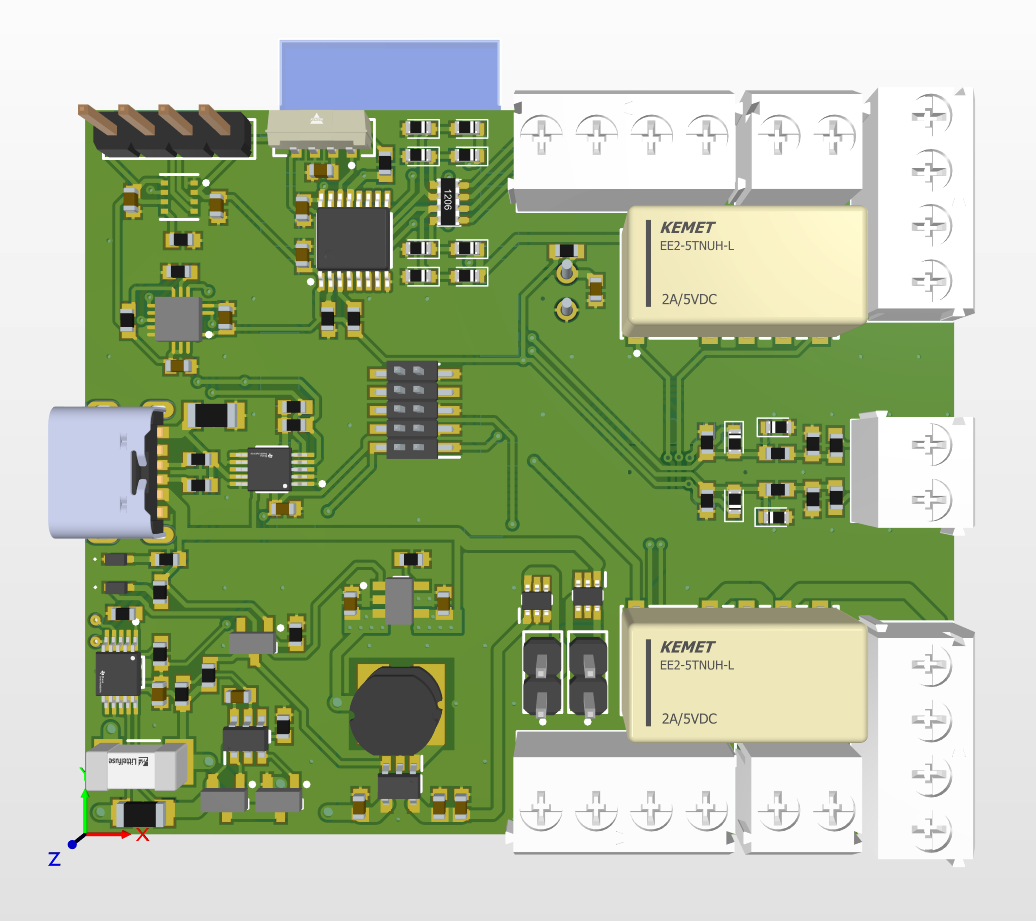
\includegraphics[width=\textwidth]{img/powerboardpcbkesz.png}
    \caption{Power Node PCB}
    \label{fig:powernodepcb}
\end{figure}
At the moment, the PCB plan is half-finished, as only the components have been installed on the 3D design so far. The panel size is going to be 50x60\,\si{\milli\metre\squared} as the chose Li-Po cell dimensions comply with it. The layout is shown in Figure \ref{fig:powernodepcb}. This plan is not realised as many of the necessary parts could not be ordered due shortages in the supply chain.